%%%%%%%%%%%%%%%%%%%%%%%%%%%%%%%%%%%%%%%%%%%%%%%%%%%%%%%%%%%%%%%%%%%%%%%
% BAB 2
%%%%%%%%%%%%%%%%%%%%%%%%%%%%%%%%%%%%%%%%%%%%%%%%%%%%%%%%%%%%%%%%%%%%%%%

\mychapter{2}{BAB 2 LANDASAN KEPUSTAKAAN}



\section{Tinjauan Pustaka}

% comments
%% comments
Beberapa referensi digunakan dalam penelitian ini. 
\textcite{pramukantoroHeartbeatClassifierContinuous2022} telah mengusulkan beberapa algoritma untuk melakukan klasifikasi detak jantung dalam penelitiannya. 
Algoritma tersebut menggunakan RR-Interval dengan 9 deskriptor sebagai fiturnya.
Penelitian tersebut menggunakan metode \textit{machine learning Decision Tree, Gradient Boosting, k-Nearest Neighbors, Multi-layer Perceptron, Random Forest}, dan \textit{Support Vector Machine}, serta model \textit{deep learning} berupa \textit{Artificial Neural Network} (ANN). 
Penelitian tersebut mencapai nilai akurasi 99,31\% dengan menggunakan metode \textit{decision tree}, serta teknik \textit{random oversampling} untuk menambah jumlah sampel.
Selain itu, penelitian tersebut juga melakukan eksperimen implementasi inferensi secara \textit{realtime} untuk memprediksi kesehatan pasien dan mencapai hasil yang baik.

% Pada penelitian lain, \textcite{mondejar-guerraHeartbeatClassificationFusing2019} mengusulkan algoritma klasifikasi detak jantung dengan menggunakan fitur RR-Interval dengan 8 deskriptor. Dengan menggunakan fitur RR-Interval dan metode SVM, penelitian tersebut mendapatkan nilai akurasi 76,2\%. Penelitian tersebut juga menggunakan metode \textit{ensemble} SVM dengan fitur gabungan RR-Interval, wavelet, dan \textit{higher order statistics} (HOS) dan mendapat nilai akurasi 94,5\%.

Pada penelitian lain, \textcite{shchetininArrhythmiaDetectionUsing2022} telah melakukan penelitian untuk melakukan klasifikasi detak jantung dengan menggunakan metode \textit{deep learning} \textit{Long Short-Term Memory} (LSTM). 
Penelitian tersebut menggunakan dataset MIT-BIH Arrhythmia Database dan melakukan klasifikasi detak jantung menjadi 5 kelas, yaitu N, SVEB, VEB, F, dan Q.
Penelitian tersebut membuktikan bahwa metode LSTM digabungkan dengan teknik \textit{oversampling} SMOTE ENN dapat melakukan klasifikasi detak jantung dengan akurasi 97,22\%. 
% Pada penelitian lain, \textcite{shchetininArrhythmiaDetectionUsing2022} telah membuktikan bahwa metode LSTM dapat digunakan untuk melakukan klasifikasi detak jantung dan mendapatkan hasil yang baik.
% Penelitian tersebut melakukan klasifikasi detak jantung menjadi 5 kelas, yaitu N, SVEB, VEB, F, dan Q.

Pada penelitian sebelumnya, \textcite{sururiComparisonSeveralWavelet2023} telah melakukan perbandingan beberapa metode \textit{wavelet} sebagai metode ekstraksi fitur untuk inferensi klasifikasi detak jantung. 
Penelitian tersebut menggunakan metode \textit{wavelet Continuous Wavelet Transform} (CWT), \textit{Discrete Wavelet Transform} (DWT), dan \textit{Stationary Wavelet Transform} (SWT) untuk melakukan ekstraksi fitur dan digabungkan dengan metode \textit{deep learning Convolutional Neural Network} (CNN) untuk melakukan klasifikasi detak jantung menjadi 5 kelas.
Penelitian tersebut juga melakukan pengujian inferensi menggunakan dataset primer sepanjang 30 menit untuk mengevaluasi performa inferensi model klasifikasi detak jantung.
Penelitian tersebut mendapatkan hasil bahwa metode CWT memberikan nilai akurasi tertinggi, yaitu 99,08\%, namun memiliki waktu inferensi yang paling lama, yaitu 21,1326 detik dan penggunaan memori yang paling tinggi, yaitu 656,02 MB.
Sementara itu, metode DWT memberikan nilai akurasi terendah, yaitu 96,70\%, namun memiliki waktu inferensi tercepat, yaitu 12,9248 detik dan penggunaan memori terendah, yaitu 109,98 MB.

% \cite{FALASCHETTI20223479} & LSTM & STM32L4 (ARM Cortex-M4) & 0.9019 & 665.86\\
%
% \cite{liEnablingOndeviceClassification2021} & 1-D CNN & Raspberry Pi Zero & 0.9835 & 7.08\\
%
% \cite{heLiteNetLightweightNeural2018} & LiteNet & Intel Core i3-2370M & 0.9787 & \tilde 25\\
%
% \cite{abayaratneRealTimeCardiacArrhythmia2019} & RNN-LSTM & - & 0.947 & 6.88\\
%
% \cite{mhamdiArtificialIntelligenceCardiac2022} & MobileNetV2 & Raspberry Pi 4 B & 0.94 & 160\\
Selain itu, masih terdapat beberapa penelitian lain yang telah dilakukan oleh peneliti lain terkait inferensi klasifikasi detak jantung.
Dalam penelitiannya, \textcite{saadatnejadLSTMBasedECGClassification2020} telah mengimplementasikan model LSTM untuk melakukan klasifikasi detak jantung dan mendapat akurasi 97,41\% serta waktu inferensi 31,2 ms.
Dalam penelitian lain, \textcite{9878113} berhasil melakukan klasifikasi detak jantung dengan menggunakan gabungan CNN 1D dan 2D dan mendapat akurasi 99,1\% serta waktu inferensi 9 ms.
Selanjutnya, \textcite{FALASCHETTI20223479} telah mengimplementasikan model LSTM untuk klasifikasi detak jantung pada STM32L4 (ARM Cortex-M4) dan mendapat akurasi 90,19\% serta waktu inferensi 665,86 ms.
Kemudian, \textcite{liEnablingOndeviceClassification2021} telah mengimplementasikan model 1-D CNN
untuk klasifikasi detak jantung
pada Raspberry Pi Zero dan mendapat akurasi 98,35\% serta waktu inferensi 7,08 ms.
\textcite{heLiteNetLightweightNeural2018} telah mengimplementasikan model LiteNet untuk klasifikasi detak jantung pada Intel Core i3-2370M dan mendapat akurasi 97,87\% serta waktu inferensi sekitar 25 ms.
\textcite{abayaratneRealTimeCardiacArrhythmia2019} telah mengimplementasikan model RNN-LSTM untuk klasifikasi detak jantung dan mendapat akurasi 94,7\% serta waktu inferensi 6,88 ms.
\textcite{mhamdiArtificialIntelligenceCardiac2022} telah mengimplementasikan model MobileNetV2 untuk klasifikasi detak jantung pada Raspberry Pi 4 B dan mendapat akurasi 94\% serta waktu inferensi 160 ms.


\section{Landasan Teori}

% \subsection{Detak Jantung}
% \label{subsec: landasan-detak-jantung}



% mitbih

\subsection{\emph{Electrocardiogram} (ECG)}
\label{subsec: landasan-ecg}

\textit{Electrocardiogram} (ECG) merupakan uji kardiologi yang umum dilakukan untuk merekam aktivitas listrik jantung selama suatu periode dengan menggunakan elektroda \parencite{yoonDeepLearningbasedElectrocardiogram2019}.
Elektroda tersebut mendeteksi perubahan listrik kecil yang disebabkan oleh depolarisasi dan repolarisasi otot jantung pada tiap detaknya.
Hasil dari ECG tersebut berupa gelombang yang dapat digunakan untuk diagnosis medis.
ECG dapat digunakan untuk berbagai tujuan, seperti mengukur konsistensi, ukuran, dan lokasi denyut jantung serta untuk mengidentifikasi kerusakan jantung.


Gambar \ref{fig: ecg-morphology} menunjukkan morfologi gelombang ECG. ECG terdiri dari beberapa komponen: gelombang P, kompleks QRS, dan gelombang T, serta durasi antara komponen tersebut \parencite{anbalaganAnalysisVariousTechniques2023}.  Gelombang P menunjukkan depolarisasi atrium, kompleks QRS menunjukkan depolarisasi ventrikel, dan gelombang T menunjukkan repolarisasi ventrikel.

\begin{figure}[H]
  \centering
  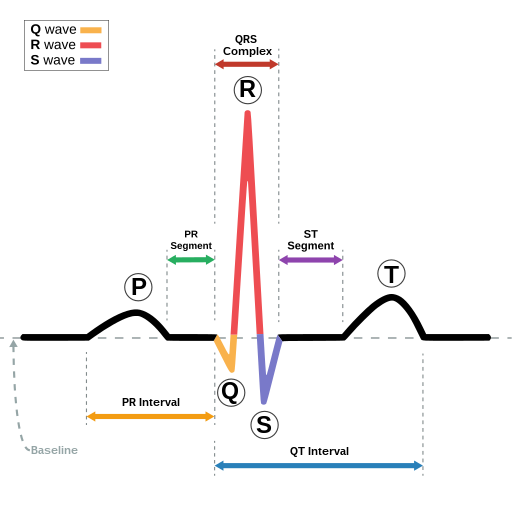
\includegraphics[width=.5\linewidth]{img/ecg-morphology.png}
  \caption{Morfologi gelombang ECG}
  Sumber: \textcite{wiki:xxx}
  \label{fig: ecg-morphology}
\end{figure}

% rri
% Cardiovascular Physiology
% Paola A. Lanfranchi, Virend K. Somers, in Principles and Practice of Sleep Medicine (Fifth Edition), 2011
%
% Heart Rate, Arterial Blood Pressure, and Their Variability
% RR interval, the time elapsed between two successive R-waves of the QRS signal on the electrocardiogram (and its reciprocal, the HR) is a function of intrinsic properties of the sinus node as well as autonomic influences. Blood pressure is a function of vascular resistance (an expression of arterial constriction or dilation) and cardiac output (the blood volume being pumped by the heart in 1 minute), which is a function of HR, cardiac contractility, and diastolic blood volume, all components controlled in part by the autonomic nervous system.

\subsection{RR-Interval}
\label{subsec: landasan-rri}

RR-Interval adalah jarak waktu antara dua puncak 'R' pada sinyal QRS dalam ECG \parencite{lanfranchiChapter20Cardiovascular2011}.
RR-Interval merupakan salah satu fitur utama dalam analisis detak jantung.
Visualisasi dari RR-Interval ditunjukkan oleh Gambar \ref{fig:rri}.
Dalam gambar tersebut, terdapat puncak 'R' yang menandakan titik maksimum voltase selama siklus detak jantung pada sinyal ECG.
% Jarak antara dua puncak 'R' ini menunjukkan RR-Interval yang menjadi fitur utama dalam penelitian ini.
Jarak antara dua puncak 'R' ini menunjukkan RR-Interval.
\begin{figure}[H]
  \centering
  % \includegraphics[scale=.7]{img/lstm-Page-7.drawio.pdf}
  \fbox{\includegraphics[width=.7\linewidth]{img/lstm-Page-7.drawio.pdf}}
  \caption{RR-Interval}
  \label{fig:rri}
\end{figure}

% ectopic beats
\subsection{Detak \textit{Ectopic}}
\label{subsec: landasan-ectopic}

% Ectopic beats are extra beats that arise from an abnormal site that is different from the normal pacemaker of the heart (the sinus node). Ectopic beats can be thought of as extra electrical impulse that originate from an abnormal ‘switch’. Therefore, in a patient with ectopic beats, after every few beats from natural pacemaker (the sinus node ‘switch’), an extra beat will fire off from the abnormal site (ectopic ‘switch’). The extra beat typically occurs a short time after a normal beat and is therefore commonly referred to as a premature ectopic beat. In the majority of cases, the abnormal ‘switch’ fires off in a random fashion and therefore the heart does not beat in a synchronized fashion.
%
% Ectopic beats may arise from multiple locations in the heart. Extra beats that arise from the top chambers of the heart (atria) are called supraventricular ectopic beats (or premature supraventricular ectopic beats). Extra beats arising from the lower chambers (ventricles) are known as ventricular ectopic beats (or premature ventricular ectopic beats).

% Ectopic beats are abnormal beats that are due to unusual impulses. These abnormal excitations originate from atrio-ventricular junction or ventricles rather than the sino-atrial node. Ectopic beats can be seen in the ECG signal as abnormal waveforms.

% Ectopic heartbeats are changes in a heartbeat that is otherwise normal. These changes lead to extra or skipped heartbeats. 
% Ectopic beats may be caused or made worse by smoking, alcohol use, caffeine, stimulant medicines, and some street drugs.


Menurut kamus \textcite{merriam-websterDefinitionECTOPIC2024}, istilah \textit{ectopic} mengacu pada kejadian yang terjadi pada posisi yang tidak normal.
% Menurut kamus \textcite{merriam-websterDefinitionECTOPIC2024}, istilah \textit{ectopic} memiliki arti terjadi pada posisi yang tidak normal.
Detak \textit{ectopic} atau \textit{ectopic beats} adalah detak jantung abnormal yang terjadi di luar ritme detak jantung normal.
% Detak jantung normalnya dipacu secara alami oleh \textit{nodus sinoatrial} (SA).
Detak jantung normalnya dipacu oleh \textit{nodus sinoatrial} (SA), sebuah struktur di jantung yang berfungsi untuk memacu detak jantung secara alami.
Namun, detak \textit{ectopic} terjadi ketika impuls listrik yang memacu detak jantung bukan berasal dari SA, melainkan dari tempat lain di dalam jantung \parencite{mahidasaagarEctopicBeats}.
Detak \textit{ectopic} dapat berasal dari serambi jantung (atrium) maupun bilik jantung (ventrikel).
Detak \textit{ectopic} yang berasal dari atrium disebut dengan \textit{supraventricular ectopic beats}, sedangkan detak \textit{ectopic} yang berasal dari ventrikel disebut dengan \textit{ventricular ectopic beats}.
Detak \textit{ectopic} dapat dikenali melalui pola gelombang yang tidak normal pada sinyal \textit{electrocardiogram} (ECG).
% \subsubsection{\textit{Supraventricular Ectopic Beats} (SVEB)}
% \label{subsubsec: landasan-sveb}
%
% \subsubsection{\textit{Ventricular Ectopic Beats} (VEB)}
% \label{subsubsec: landasan-veb}

\subsection{\textit{MIT-BIH Arrhythmia Database}}
\label{subsec: landasan-mitbih}

% \textit{MIT-BIH Arrhythmia Database} adalah dataset publik yang berisi rekaman ECG dari 47 pasien yang berdurasi 30 menit \parencite{moodyImpactMITBIHArrhythmia2001}.
\textit{MIT-BIH Arrhythmia Database} merupakan salah satu dataset publik yang dikembangkan oleh \textit{Massachusetts Institute of Technology} (MIT) dan \textit{Beth Israel Hospital} (BIH) \parencite{moodyImpactMITBIHArrhythmia2001}.
MIT-BIH Arrhythmia Database menjadi salah satu dataset standar yang banyak digunakan dalam penelitian terkait analisis sinyal ECG.
Dataset ini berisi 48 rekaman ECG dari 47 pasien yang masing-masing berdurasi 30 menit dan terdiri dari dua kanal.
Dari 48 rekaman tersebut, data 102, 104, 107, dan 217 berisi data detak jantung yang sedang dipacu.
Dataset ini direkam dengan frekuensi 360 Hz dan resolusi 11-bit.
Setiap detak jantung pada dataset, telah diberi label dan anotasi oleh para ahli.
% Pemberian label pada detak jantung dilakukan dengan menggunakan simbol-simbol tertentu.
% Simbol-simbol tersebut dideskripsikan pada tabel \ref{tab:beat_symbols}.
Pemberian label dilakukan menggunakan simbol-simbol tertentu yang dijelaskan dalam Tabel \ref{tab:beat_symbols}.

% tabel simbol yang digunakan pada dataset

% Symbol	Meaning
% · or N	Normal beat
% L	Left bundle branch block beat
% R	Right bundle branch block beat
% A	Atrial premature beat
% a	Aberrated atrial premature beat
% J	Nodal (junctional) premature beat
% S	Supraventricular premature beat
% V	Premature ventricular contraction
% F	Fusion of ventricular and normal beat
% [	Start of ventricular flutter/fibrillation
% !	Ventricular flutter wave
% ]	End of ventricular flutter/fibrillation
% e	Atrial escape beat
% j	Nodal (junctional) escape beat
% E	Ventricular escape beat
% /	Paced beat
% f	Fusion of paced and normal beat
% x	Non-conducted P-wave (blocked APB)
% Q	Unclassifiable beat
% |	Isolated QRS-like artifact

\begin{table}[H]
    \centering
    \caption{Deskripsi simbol pada \textit{MIT-BIH Arrhythmia Database}}
    \begin{tabular}{| @{\hspace{2em}} c @{\hspace{2em}} | l |}
    \hline
    % \textbf{Simbol} & {\centering \textbf{Deskripsi}} \\
    \multicolumn{1}{|c|}{\textbf{Simbol}} & \multicolumn{1}{c|}{\textbf{Deskripsi}} \\
    \hline
    % $\cdot$ or N & Normal beat \\
    $\cdot$ atau N & Denyut normal \\
    \hline
    % L & Left bundle branch block beat \\
    L & Denyut \textit{left bundle branch block} (LBBB) \\
    \hline
    % R & Right bundle branch block beat \\
    R & Denyut \textit{right bundle branch block} (RBBB) \\
    \hline
    % A & Atrial premature beat \\
    A & \textit{Atrial premature beat} (APB) \\
    \hline
    % a & Aberrated atrial premature beat \\
    a & \textit{Aberrated atrial premature beat} \\
    \hline
    % J & Nodal (junctional) premature beat \\
    J & \textit{Nodal (junctional) premature beat} \\
    \hline
    % S & Supraventricular premature beat \\
    S & \textit{Supraventricular premature beat} \\
    \hline
    % V & Premature ventricular contraction \\
    V & \textit{Premature ventricular contraction} (PVC) \\
    \hline
    % F & Fusion of ventricular and normal beat \\
    F & Gabungan denyut ventrikel dan normal \\
    \hline
    % {[} & Start of ventricular flutter/fibrillation \\
    {[} & Awal dari \textit{ventricular flutter/fibrillation} \\
    \hline
    % ! & Ventricular flutter wave \\
    ! & \textit{Ventricular flutter wave} \\
    \hline
    % {]} & End of ventricular flutter/fibrillation \\
    {]} & Akhir dari \textit{ventricular flutter/fibrillation} \\
    \hline
    % e & Atrial escape beat \\
    e & \textit{Atrial escape beat} \\
    \hline
    % j & Nodal (junctional) escape beat \\
    j & \textit{Nodal (junctional) escape beat} \\
    \hline
    % E & Ventricular escape beat \\
    E & \textit{Ventricular escape beat} \\
    \hline
    % / & Paced beat \\
    / & Denyut yang dipacu \\
    \hline
    % f & Fusion of paced and normal beat \\
    f & Gabungan denyut dipacu dan normal \\
    \hline
    % x & Non-conducted P-wave (blocked APB) \\
    x & Gelombang P yang tidak terkonduksi \\
    \hline
    % Q & Unclassifiable beat \\
    Q & Denyut yang tidak dapat diklasifikasikan \\
    % | & Isolated QRS-like artifact \\
    \hline
    \end{tabular} \\
    \vspace{0.5em}
    Sumber: \textcite{moodyImpactMITBIHArrhythmia2001}
    \label{tab:beat_symbols}
\end{table}

\subsection{\textit{Long Short-Term Memory} (LSTM)}
\label{subsec: landasan-lstm}

\textit{Long Short-Term Memory} atau dapat disingkat LSTM merupakan pengembangan dari metode \textit{deep learning Recurrent Neural Network} (RNN). LSTM dirancang untuk mengatasi salah satu masalah yang umum terjadi pada RNN tradisional, yaitu hilangnya informasi masa lalu \parencite{hochreiterLongShorttermMemory1997}. Metode LSTM dapat diterapkan pada klasifikasi, pengolahan, dan prediksi berdasarkan data sekuensial, seperti teks dan suara,  termasuk juga data yang terkait dengan bidang kesehatan.

\begin{figure}[H]
  \centering
  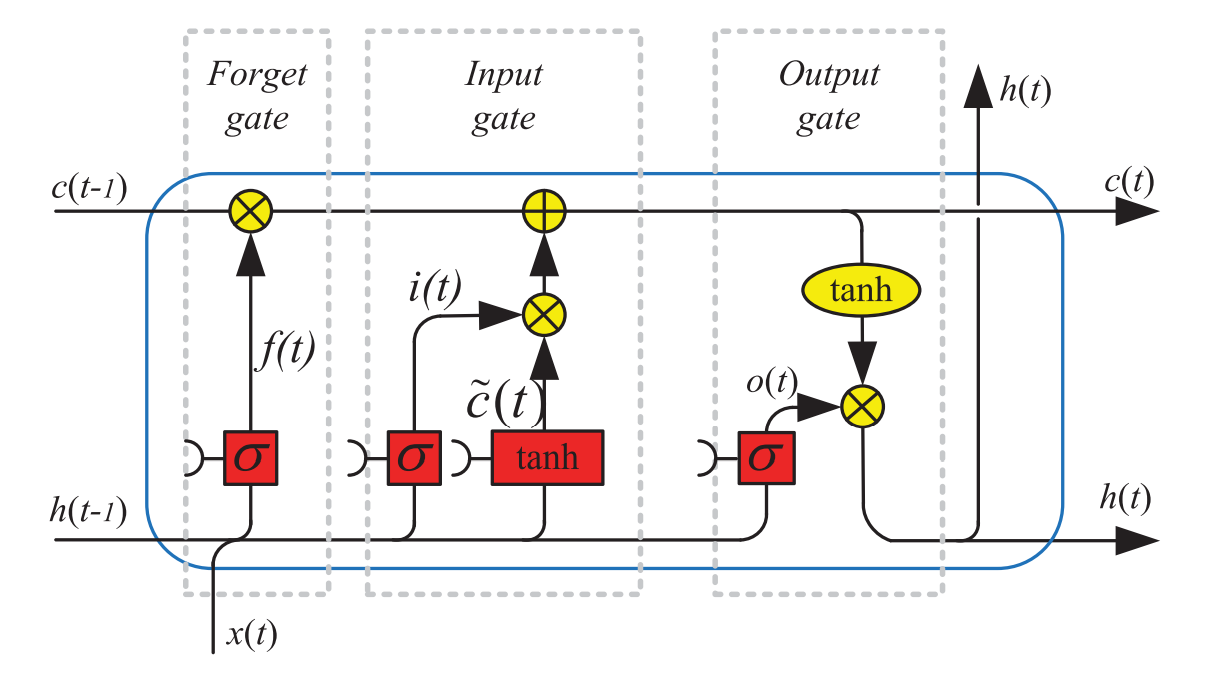
\includegraphics[width=.8\linewidth]{img/ecg-arch.png}
  \caption{Arsitektur sel LSTM}
  Sumber: \textcite{yuReviewRecurrentNeural2019}
  \label{fig:arsitektur-lstm}
\end{figure}

Gambar \ref{fig:arsitektur-lstm} menunjukkan arsitektur sel LSTM. Sebuah sel LSTM umumnya terdiri dari tiga buah \textit{gate}, yaitu \textit{input gate, output gate}, dan \textit{forget gate}. Ketiga gate tersebut berfungsi untuk mengatur informasi yang masuk maupun keluar dari sel LSTM.
\textit{Input gate} menentukan informasi baru yang akan disimpan pada \textit{cell state} (Ct), \textit{output gate} menentukan informasi apa yang akan jadi output, dan \textit{forget gate} menentukan informasi apa yang akan dibuang dari \textit{cell state} \parencite{yuReviewRecurrentNeural2019}.

Berdasarkan Gambar \ref{fig:arsitektur-lstm}, secara matematis LSTM dapat didefinisikan dengan persamaan \ref{def-lstm}
\begin{equation}
\begin{split}
    f_t &= \sigma (W_{fh}h_{t-1} + W_{fx}x_t + b_f), \\
    i_t &= \sigma (W_{ih}h_{t-1} + W_{ix}x_t + b_i),\\
    \tilde{c}_t &= \tanh (W_{\tilde{c}h}h_{t-1} + W_{\tilde{c}x}x_t + b_{\tilde{c}}), \\
    c_t &= f_t \cdot c_{t-1}+ i_t \cdot \tilde{c}_t,\\
    o_t &= \sigma (W_{oh}h_{t-1} + W_{ox}x_t + b_o), \\
    h_t &= o_t \cdot \tanh(c_t).
\end{split}
    \label{def-lstm}
\end{equation}
\noindent
dengan \(f_t\), \(i_t\), \(o_t\) dan \(c_t\) masing-masing menunjukkan nilai \emph{forget gate}, \emph{input gate}, \emph{output gate}, dan \emph{cell state}.

\subsection{Perangkat Tepi (\emph{Edge Device})}
\label{subsec: landasan-edge-device}
% Referensi: \cite{khouasTrainingMachineLearning2024}
% Edge Computing (EC) is a new computing paradigm that aims to address the limitations of traditional Cloud Computing models in handling large scale data generated by the increasing number of smart devices connected to the Internet. It involves performing calculations at the edge of the network, closer to the user and the source of the data. EC emphasizes local, small-scale data storage and processing, providing benefits such as reduced bandwidth load, faster response speed, improved security, and enhanced privacy compared to traditional Cloud Computing models [2].
%
% Edge Computing addresses several limitations of Cloud Computing, that stem from the frequent communications needed between end/edge devices and cloud server, in the standard Cloud Computing paradigm and the reliance of storing data centrally, which might compromise the privacy or security of sensible data.
%
% • Reduced latency: EC brings data processing closer to the source, reducing the time it takes for data to travel to a centralized cloud server, thereby reducing latency and improving response times [3].
% • Bandwidth optimization: EC reduces the need for transmitting large amounts of data to centralized cloud servers, resulting in reduced bandwidth load and reduced network congestion [2].
% • Improved data privacy: EC allows for local data processing, reducing the need to transmit sensitive data to centralized cloud servers, thereby minimizing the risk of data breaches and unauthorized access [2].
% • Operational resilience: EC enables applications to continue functioning even in disconnected or low-bandwidth environments, ensuring operational resilience and reducing dependency on a centralized cloud infrastructure [3].
Perangkat tepi (\emph{edge device}) merupakan perangkat yang berada di tepi atau
ujung jaringan yang berfungsi untuk melakukan pemrosesan data secara lokal \parencite{khouasTrainingMachineLearning2024}.
Berbeda dengan model komputasi awan tradisional, perangkat tepi melakukan pemrosesan data di dekat pengguna dan sumber data.
% Perangkat tepi melakukan pemrosesan data di dekat pengguna dan sumber data
% , sehingga dapat memberikan keuntungan seperti beban bandwidth yang lebih rendah, kecepatan respon yang lebih cepat, keamanan yang lebih baik, dan privasi yang lebih terjamin dibandingkan dengan model komputasi awan tradisional.
% Perangkat tepi umumnya memiliki keterbatasan sumber daya, seperti daya komputasi dan memori.
Perangkat ini sering digunakan untuk aplikasi yang membutuhkan respon cepat, seperti pemantauan kesehatan.

Perangkat tepi memiliki beberapa kelebihan apa bila dibandingkan dengan komputasi awan tradisional, seperti:
\begin{enumerate}
    \item Latensi yang lebih rendah: Posisi perangkat tepi yang berdekatan dengan sumber data menghilangkan waktu yang dibutuhkan untuk mentransmisikan data ke peladen awan.
    % \item Optimisasi bandwidth: Perangkat tepi mengurangi kebutuhan untuk mentransmisikan data dalam jumlah besar ke server awan pusat, sehingga mengurangi beban bandwidth dan kemacetan jaringan.
    \item Privasi data yang lebih baik: Perangkat tepi memungkinkan pemrosesan data secara lokal, sehingga mengurangi risiko terjadinya kebocoran data dan akses yang tidak sah.
    \item Biaya operasional yang lebih rendah: Pemrosesan data di perangkat tepi tidak memerlukan biaya langganan layanan awan serta memungkinkan aplikasi berjalan tanpa jarigan internet.
\end{enumerate}

Meskiput memiliki beberapa kelebihan, perangkat tepi juga memiliki beberapa keterbatasan.
Perangkat tepi umumnya memiliki sumber daya yang terbatas, seperti daya komputasi dan memori.
Oleh karena itu, model yang diimplementasikan pada perangkat tepi harus dioptimalkan agar dapat berjalan dengan baik pada perangkat tersebut.
Keterbatasan sumber daya perangkat tepi juga menyebabkan keterbatasan jumlah proses yang dapat dijalankan secara bersamaan.

\subsection{Raspberry Pi 4 Model B}
\label{subsec: landasan-raspi}
%
%raspi secara umum
Raspberry Pi merupakan sebuah komputer mini seukuran kartu kredit yang dikembangkan oleh Raspberry Pi Foundation \parencite{8756967}. 
Raspberry Pi memiliki beberapa kelebihan, seperti ukurannya yang kecil, konsumsi daya yang rendah, harga yang terjangkau, serta kemampuan komputasi baik.
%need citation
Raspberry Pi dapat diaplikasikan pada berbagai bidang, seperti industri, agrikultur, bioteknologi, dan kesehatan \parencite{9760691}.

% %raspi 4 
% %*sekara sudah bukan yang terbaru, sudah ada raspi 5
Raspberry Pi 4 model B merupakan salah satu varian dari Raspberry Pi generasi keempat.
% Raspberry Pi 4 model B memiliki spesifikasi prosesor \textit{quad-core} ARM Cortex-A72 1.5GHz, dengan pilihan RAM 2GB, 4GB, atau 8GB LPDDR4-3200 SDRAM. Raspberry Pi 4 model B juga dilengkapi dengan konektivitas WiFi 2.4GHz dan 5GHz, Bluetooth 5.0, serta \textit{ethernet} dengan kecepatan maksimum 1Gbps. Raspberry Pi 4 model B juga memiliki \textit{port micro} HDMI, USB 3.0, USB 2.0, dan port GPIO.
% • Broadcom BCM2711, Quad core Cortex‐A72 (ARM v8) 64‐bit SoC @ 1.8GHz
% • 1GB, 2GB, 4GB or 8GB LPDDR4‐3200 SDRAM (depending on model)
% • 2.4 GHz and 5.0 GHz IEEE 802.11ac wireless, Bluetooth 5.0, BLE
% • Gigabit Ethernet
% • 2 USB 3.0 ports; 2 USB 2.0 ports.
% • Raspberry Pi standard 40 pin GPIO header (fully backwards compatible with
% previous boards)
% • 2 × micro‐HDMI® ports (up to 4kp60 supported)
% • 2‐lane MIPI DSI display port
% • 2‐lane MIPI CSI camera port
% • 4‐pole stereo audio and composite video port
% • H.265 (4kp60 decode), H264 (1080p60 decode, 1080p30 encode)
% • OpenGL ES 3.1, Vulkan 1.0
% 12• Micro‐SD card slot for loading operating system and data storage
% • 5V DC via USB‐C connector (minimum 3A*)
% • 5V DC via GPIO header (minimum 3A*)
% • Power over Ethernet (PoE) enabled (requires separate PoE HAT)
% • Operating temperature: 0 – 50 degrees C ambient
Raspberry Pi 4 model B memiliki spesifikasi sebagai berikut:
\begin{itemize}
  \item \textit{Chipset} Broadcom BCM2711, \textit{quad-core} Cortex-A72 (ARM v8) 64-bit SoC @ 1.8GHz.
  \item RAM 2GB, 4GB, atau 8GB LPDDR4-3200 SDRAM (tergantung model).
  \item Konektivitas WiFi 2.4GHz dan 5GHz, Bluetooth 5.0, serta \textit{ethernet} dengan kecepatan maksimum 1Gbps.
  \item \textit{Port} micro-HDMI, USB 3.0, USB 2.0, dan \textit{port} GPIO.
\end{itemize}
%
% % raspi 3
% % Pengujian dilakukan pada perangkat Raspberry Pi 3B. Perangkat ini memiliki prosesor ARMv8 quad-core 1,2GHz dan RAM 1GB LPDDR2. Konektivitas perangkat ini didukung dengan 2.4Ghz WiFi serta \textit{ethernet} dengan kecepatan maksimum 100Mbps.
% Raspberry Pi 3 merupakan salah satu varian dari Raspberry Pi generasi ketiga. Raspberry Pi 3 memiliki spesifikasi prosesor ARMv8 \textit{quad-core} 1,2GHz dan RAM 1GB LPDDR2. Raspberry Pi 3 juga telah dilengkapi dengan konektivitas WiFi 2.4GHz dan \textit{ethernet} dengan kecepatan maksimum 100Mbps. Raspberry Pi 3 juga memiliki \textit{port} HDMI, USB 2.0, dan \textit{port} GPIO.

% intel nuc
\subsection{Intel NUC}
\label{subsec: landasan-nuc}
Intel NUC (\textit{Next Unit of Computing}) merupakan lini produk komputer dengan ukuran kecil yang dikembangkan oleh Intel \parencite{bhismasidartoReviewNextUnit2013}.
Intel NUC memiliki beberapa kelebihan, seperti ukurannya yang kecil dan konsumsi daya yang rendah.
Pada umumnya, Intel NUC memiliki ukuran board sebesar 4x4 inci.
Meskipun memiliki ukuran yang kecil, Intel NUC memiliki performa yang baik, tidak berbeda dengan komputer desktop pada umumnya.

Pada penelitian ini, digunakan Intel NUC dengan model NUC11PAHi3.
Intel NUC NUC11PAHi3 memiliki spesifikasi sebagai berikut:
\begin{itemize}
  \item Prosesor Intel Core i3-1115G4, \textit{dual-core} 3.0GHz.
  \item RAM hingga 64GB DDR4-3200 SDRAM.
  \item \textit{Port} HDMI, USB 3.0, USB 2.0, dan mini-DisplayPort.
    % 2.5 gigabit ethernet
    % wifi ax
    % bluetooth
    % tdp 40w
    % ukuran 4x4 inci
  \item Konektivitas 2.5 gigabit \textit{ethernet}, WiFi 6, dan Bluetooth.
  \item TDP 40W.
  \item Dimensi 4x4 inci.
\end{itemize}
% klasifikasi detak jantung
% tentang detak jantung menurut AAMI

% heart related disease class
% N, sveb, veb, f, dan q
% \section{Klasifikasi Detak Jantung}

% \section{Inferensi}

% metrik evaluasi
% akurasi, presisi, recall, f1-score
\subsection{Metrik Evaluasi}
\label{subsec: landasan-metrik-evaluasi}
Metrik evaluasi adalah ukuran yang digunakan untuk mengevaluasi performa model klasifikasi.
% penjelasan tp, fp, tn, fn
Terdapat empat istilah yang sering digunakan dalam metrik evaluasi, yaitu \textit{true positive} (TP), \textit{false positive} (FP), \textit{true negative} (TN), dan \textit{false negative} (FN).
\textit{True positive} (TP) adalah jumlah sampel positif yang diklasifikasikan dengan benar, sedangkan \textit{false positive} (FP) adalah jumlah sampel negatif yang salah diklasifikasikan sebagai positif.
Begitu pula dengan \textit{true negative} (TN) yang merupakan jumlah sampel negatif yang diklasifikasikan dengan benar dan \textit{false negative} (FN) yang merupakan jumlah sampel positif yang salah diklasifikasikan sebagai negatif.
% \begin{itemize}
%     \item \textit{True positive} (TP) adalah jumlah sampel positif yang diklasifikasikan dengan benar.
%     \item \textit{False positive} (FP) adalah jumlah sampel negatif yang salah diklasifikasikan sebagai positif.
%     \item \textit{True negative} (TN) adalah jumlah sampel negatif yang diklasifikasikan dengan benar.
%     \item \textit{False negative} (FN) adalah jumlah sampel positif yang salah diklasifikasikan sebagai negatif.
% \end{itemize}

Terdapat beberapa metrik evaluasi yang umum digunakan dalam klasifikasi, seperti akurasi, presisi, \textit{recall}, dan \textit{F1-score}.
Masing-masing metrik evaluasi tersebut memberikan informasi yang berbeda mengenai performa model klasifikasi.
\subsubsection{Akurasi}
\label{subsubsec: landasan-akurasi}
% Accuracy (ACC)
%
% The accuracy is the ratio between the correctly classified samples and the total number of samples in the evaluation dataset. This metric is among the most commonly used in applications of ML in medicine, but is also known for being misleading in the case of different class proportions since simply assigning all samples to the prevalent class is an easy way of achieving high accuracy. The accuracy is bounded to [0, 1], where 1 represents predicting all positive and negative samples correctly, and 0 represents predicting none of the positive or negative samples correctly.
% ACC=#correctlyclassifiedsamples#allsamples=TP+TNTP+FP+TN+FN
% 3
Akurasi adalah rasio antara jumlah sampel yang diklasifikasikan dengan benar dan total jumlah sampel pada dataset evaluasi \parencite{hicksEvaluationMetricsMedical2022}.
Akurasi merupakan salah satu metrik evaluasi yang paling umum digunakan dalam evaluasi \textit{machine learning} di bidang kesehatan.
Akurasi dapat didefinisikan dengan persamaan \ref{def-akurasi}.
\begin{equation}
    ACC = \frac{TP + TN}{TP + FP + TN + FN}.
    \label{def-akurasi}
\end{equation}

\subsubsection{Presisi}
\label{subsubsec: landasan-presisi}
% perbandingan jumlah data yang benar‐benar positif terhadap jumlah data yang diprediksi positif.
% The precision denotes the proportion of the retrieved samples which are relevant
Presisi adalah rasio antara jumlah sampel positif yang diklasifikasikan dengan benar dan jumlah sampel yang diprediksi positif.
Presisi menujukkan proporsi dari sampel yang relevan yang diambil dari sampel yang diambil \parencite{hicksEvaluationMetricsMedical2022}.
Presisi dapat didefinisikan dengan persamaan \ref{def-presisi}.
\begin{equation}
    PRE = \frac{TP}{TP + FP}.
    \label{def-presisi}
\end{equation}

\subsubsection{\textit{Recall}}
\label{subsubsec: landasan-recall}
% The recall, also known as the sensitivity or True Positive Rate (TPR), denotes the rate of positive samples correctly classified, and is calculated as the ratio between correctly classified positive samples and all samples assigned to the positive class.
% This metric is also regarded as being among the most important for medical studies, since it is desired to miss as few positive instances as possible,
\textit{Recall} adalah rasio antara jumlah sampel positif yang diklasifikasikan dengan benar dan jumlah sampel yang sebenarnya positif.
\textit{Recall} juga dikenal sebagai sensitivitas atau \textit{True Positive Rate} (TPR).
\textit{Recall} dianggap sebagai salah satu metrik evaluasi yang paling penting dalam studi medis \parencite{hicksEvaluationMetricsMedical2022}.
Semakin tinggi nilai \textit{recall}, semakin sedikit sampel positif yang salah diklasifikasikan sebagai negatif.
\textit{Recall} dapat didefinisikan dengan persamaan \ref{def-recall}.
\begin{equation}
    REC = \frac{TP}{TP + FN}.
    \label{def-recall}
\end{equation}

\subsubsection{\textit{F1-Score}}
\label{subsubsec: landasan-f1-score}
% The F1 score is the harmonic mean of precision and recall, meaning that it penalizes extreme values of either.
% This metric is not symmetric between the classes, i.e., it depends on which class is defined as positive and negative. For example, in the case of a large positive class and a classifier biased towards this majority, the F1 score, being proportional to TP, would be high. Redefining the class labels so that the negative class is the majority and the classifier is biased towards the negative class would result in a low F1 score, although neither the data nor the relative class distribution has changed.
\textit{F1-score} merupakan gabungan antara presisi dan \textit{recall}.
\textit{F1-score} menghitung rata-rata harmonik dari presisi dan \textit{recall}.
\textit{F1-score} memberikan penalti terhadap nilai ekstrim dari presisi maupun \textit{recall} \parencite{hicksEvaluationMetricsMedical2022}.
\textit{F1-score} dapat didefinisikan dengan persamaan \ref{def-f1-score}.
\begin{equation}
    F1 = 2 \times \frac{PRE \times REC}{PRE + REC}.
    \label{def-f1-score}
\end{equation}


% TODO
% landasan teori lain
% penerapan lstm di edge device

